\section{Feedback-based congestion control}

\subsection{Feedback control packet format}

\begin{figure}[!htb]
\centering
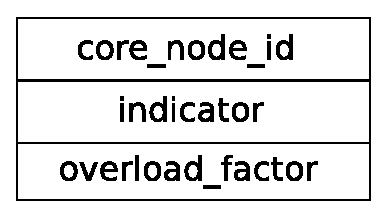
\includegraphics[width=2in]{fig/feedback_message}
\caption{Feedback Control Packet}
\label{fig:fcp}
\end{figure}

Figure \ref{fig:fcp} shows the feedback control packet fields.

core\_node\_id: indicate which core router send the feedback control packet.
Edge node can reroute to other available link according to this value.


indicator: the congestion status indicator. If congestion occurs, set to 1. Otherwise, set to 0.

overload\_factor: the percentage of burst blocked probability exceed the threshold. Edge node can determine the most congestion link with this value.

The feedback packets are broadcast to all associate ingress nodes periodically. In simulation, it is carried by a ICI format packet and assume without loss. On real network, they may transmitted within BHPs but with higher priority \cite{ref:real-network}. 

\subsection{Detection on core router}

Core routers are responsible for two main tasks: monitoring incoming bursts, broadcasting feedback control packet to the edge nodes.

The study of \cite{ref:long-term-detect} suggest multiple statistics improve estimation accuracy and react quickly. After balance the complexity and accuracy. I adopt the single statistic estimation algorithm. That is:

\begin{eqnarray*}
    B_{avg}(t) ~=~ (1-\alpha) \times B_{avg}(t-1) + \alpha \times B(t) \\
    0<\alpha<1
\end{eqnarray*}

Let $B_{avg}(t)$ denote the average data burst blocked probability of the samples at time $t$ with memory factor $\alpha$, where $B(t)$ is the current data burst blocked probability in a sample period $\tau$.

Then, the detection based on single statistic is,

\begin{enumerate}
\item if $B_{avg}(t) \geq B_{th}$, then congestion occurs 
\item otherwise, congestion clear out
\end{enumerate}

The implementation of this monitor can be found at \cite{ref:monitor}.

\subsection{Reaction on edge router}

The edge routers are responsible for receiving feedback congestion packet and adjust transmission rate inject into network through leaky bucket traffic shaping. As we know, each ingress router contains flow classifier, burst generation queue, leaky-bucket traffic shaper. Arriving BHPs move into corresponding burst queue according to their destination. 

Transmission rate are decided at the leaky bucket traffic shaper based on the feedback control packet at every core routers. For a given path, an optimal transmission rate is determined by the most-congested node on the path. 

$$
     R_{j,k}(i)=\left\{
                    \begin{aligned}
                     R_{j,k}(i-1) \times (1 + a) \quad B(i) \geq B_{th}\\
                     R_{j,k}(i-1) \times (1 - b) \quad B(i) < B_{th}
                    \end{aligned}
\right.
$$

Let $R_{i}$ denote the transmission rate of a certain path at the $i$th period. Where $a$ is the rate increasing factor and $b$ is the rate decreasing factor. Generally, $0<a<b<1$.  


The implementation of this leaky bucket rate controller can be found at \cite{ref:leaky-bucket}. 

\subsection{Determine parameter}

As the study of \cite{ref:feedback-based} suggest, the feedback mechanism and the parameter setup is very high relevant. So we need to determine the system parameter very carefully. In this part, I will explain how to determine the congestion threshold value and detect period.

Assume the inter-arrival time and service time of data burst meet the poisson distribution. Every fiber line contain $m$ available wavelength. The average arrival rate of DB is $\lambda$. The serve rate is $\mu$. Assume any input port DB scheduled to any wavelength of any output port. Thus, the output port can be considered as \verb|M/M/m/m| queueing system. Denote the traffic load $A=m\rho=m\frac{\lambda}{\mu}$. We can calculate the corresponding theory block probability according to
\verb|Erlang-B| formula. 

$$
    P_{block} ~=~ \frac{\frac{A^m}{m!}}{\sum_{i=0}^{m}\frac{A^i}{i!}}
$$

We can test this in single node value, When network load scale factor is 0.8, $\rho=1.2$, $m=10$, $P_{block} = 0.10$, when network load scale factor is 1.0, $\rho=1.5$, $P_{block} = 0.136$. We can find that is very closed to simulation result. As we know, if the congestion threshold value too low, it will impact the performance of network. On the opposite side, if this value is too high, the mechanism is restricted. So we can estimate the threshold value base this formula for
performance trade-off.  

Another important parameter is the period of detection and feedback. If this value low, the number of feedback control packets will increase and the performance of network will jitter sharply. If this time window last longer, the react of edge node will be slow. In this paper, I determine this value base on the end-to-end delay. That is 

$$ \tau = kT_{ete} $$

Where $T_{ete}$ is end-to-end delay. $\tau$ is the sampling period. For single node scenario, let $k=1000$. Through simulation result, I find that work well. How to determine this value is a complex problem, the study of \cite{ref:time-window} introduce a dynamic time windows congestion control.
